\documentclass[twoside]{book}

% Packages required by doxygen
\usepackage{fixltx2e}
\usepackage{calc}
\usepackage{doxygen}
\usepackage[export]{adjustbox} % also loads graphicx
\usepackage{graphicx}
\usepackage[utf8]{inputenc}
\usepackage{makeidx}
\usepackage{multicol}
\usepackage{multirow}
\PassOptionsToPackage{warn}{textcomp}
\usepackage{textcomp}
\usepackage[nointegrals]{wasysym}
\usepackage[table]{xcolor}

% Font selection
\usepackage[T1]{fontenc}
\usepackage[scaled=.90]{helvet}
\usepackage{courier}
\usepackage{amssymb}
\usepackage{sectsty}
\renewcommand{\familydefault}{\sfdefault}
\allsectionsfont{%
  \fontseries{bc}\selectfont%
  \color{darkgray}%
}
\renewcommand{\DoxyLabelFont}{%
  \fontseries{bc}\selectfont%
  \color{darkgray}%
}
\newcommand{\+}{\discretionary{\mbox{\scriptsize$\hookleftarrow$}}{}{}}

% Page & text layout
\usepackage{geometry}
\geometry{%
  a4paper,%
  top=2.5cm,%
  bottom=2.5cm,%
  left=2.5cm,%
  right=2.5cm%
}
\tolerance=750
\hfuzz=15pt
\hbadness=750
\setlength{\emergencystretch}{15pt}
\setlength{\parindent}{0cm}
\setlength{\parskip}{3ex plus 2ex minus 2ex}
\makeatletter
\renewcommand{\paragraph}{%
  \@startsection{paragraph}{4}{0ex}{-1.0ex}{1.0ex}{%
    \normalfont\normalsize\bfseries\SS@parafont%
  }%
}
\renewcommand{\subparagraph}{%
  \@startsection{subparagraph}{5}{0ex}{-1.0ex}{1.0ex}{%
    \normalfont\normalsize\bfseries\SS@subparafont%
  }%
}
\makeatother

% Headers & footers
\usepackage{fancyhdr}
\pagestyle{fancyplain}
\fancyhead[LE]{\fancyplain{}{\bfseries\thepage}}
\fancyhead[CE]{\fancyplain{}{}}
\fancyhead[RE]{\fancyplain{}{\bfseries\leftmark}}
\fancyhead[LO]{\fancyplain{}{\bfseries\rightmark}}
\fancyhead[CO]{\fancyplain{}{}}
\fancyhead[RO]{\fancyplain{}{\bfseries\thepage}}
\fancyfoot[LE]{\fancyplain{}{}}
\fancyfoot[CE]{\fancyplain{}{}}
\fancyfoot[RE]{\fancyplain{}{\bfseries\scriptsize Generated by Doxygen }}
\fancyfoot[LO]{\fancyplain{}{\bfseries\scriptsize Generated by Doxygen }}
\fancyfoot[CO]{\fancyplain{}{}}
\fancyfoot[RO]{\fancyplain{}{}}
\renewcommand{\footrulewidth}{0.4pt}
\renewcommand{\chaptermark}[1]{%
  \markboth{#1}{}%
}
\renewcommand{\sectionmark}[1]{%
  \markright{\thesection\ #1}%
}

% Indices & bibliography
\usepackage{natbib}
\usepackage[titles]{tocloft}
\setcounter{tocdepth}{3}
\setcounter{secnumdepth}{5}
\makeindex

% Hyperlinks (required, but should be loaded last)
\usepackage{ifpdf}
\ifpdf
  \usepackage[pdftex,pagebackref=true]{hyperref}
\else
  \usepackage[ps2pdf,pagebackref=true]{hyperref}
\fi
\hypersetup{%
  colorlinks=true,%
  linkcolor=blue,%
  citecolor=blue,%
  unicode%
}

% Custom commands
\newcommand{\clearemptydoublepage}{%
  \newpage{\pagestyle{empty}\cleardoublepage}%
}

\usepackage{caption}
\captionsetup{labelsep=space,justification=centering,font={bf},singlelinecheck=off,skip=4pt,position=top}

%===== C O N T E N T S =====

\begin{document}

% Titlepage & ToC
\hypersetup{pageanchor=false,
             bookmarksnumbered=true,
             pdfencoding=unicode
            }
\pagenumbering{alph}
\begin{titlepage}
\vspace*{7cm}
\begin{center}%
{\Large A\+S\+C\+II Table \\[1ex]\large 0.\+0.\+1 }\\
\vspace*{1cm}
{\large Generated by Doxygen 1.8.13}\\
\end{center}
\end{titlepage}
\clearemptydoublepage
\pagenumbering{roman}
\tableofcontents
\clearemptydoublepage
\pagenumbering{arabic}
\hypersetup{pageanchor=true}

%--- Begin generated contents ---
\chapter{Todo List}
\label{todo}
\Hypertarget{todo}

\begin{DoxyRefList}
\item[\label{todo__todo000003}%
\Hypertarget{todo__todo000003}%
Global \hyperlink{classASCIITable_aec29916ecab019573c16364bf33d20e9}{A\+S\+C\+I\+I\+Table\+:\+:dump} (void)]write docs  
\item[\label{todo__todo000005}%
\Hypertarget{todo__todo000005}%
Global \hyperlink{classASCIITable_ac87f7ae9bbb1a3c73b7717c5b134bd0c}{A\+S\+C\+I\+I\+Table\+:\+:nline} ]check colcount / nline redundancy  
\item[\label{todo__todo000004}%
\Hypertarget{todo__todo000004}%
Global \hyperlink{classASCIITable_a6d06a2ed737f3151484c47bff7fad033}{A\+S\+C\+I\+I\+Table\+:\+:parserow} (char $\ast$mybuffer, int mncols)]write docs  
\item[\label{todo__todo000002}%
\Hypertarget{todo__todo000002}%
Global \hyperlink{classASCIITable_a5ec694dec500699648ef16693277bc22}{A\+S\+C\+I\+I\+Table\+:\+:read} (const F\+I\+LE $\ast$inf)]write docs  
\item[\label{todo__todo000001}%
\Hypertarget{todo__todo000001}%
Global \hyperlink{classASCIITable_a68a34a07ecdc249d4a48c75797320f8f}{A\+S\+C\+I\+I\+Table\+:\+:$\sim$\+A\+S\+C\+I\+I\+Table} (void)]write docs 
\end{DoxyRefList}
\chapter{Data Structure Index}
\section{Data Structures}
Here are the data structures with brief descriptions\+:\begin{DoxyCompactList}
\item\contentsline{section}{\hyperlink{classASCIITable}{A\+S\+C\+I\+I\+Table} \\*Implements basic input/output operations on ascii table dataset }{\pageref{classASCIITable}}{}
\end{DoxyCompactList}

\chapter{File Index}
\section{File List}
Here is a list of all files with brief descriptions\+:\begin{DoxyCompactList}
\item\contentsline{section}{\hyperlink{asciitable_8h}{asciitable.\+h} }{\pageref{asciitable_8h}}{}
\item\contentsline{section}{\hyperlink{defines_8h}{defines.\+h} }{\pageref{defines_8h}}{}
\item\contentsline{section}{\hyperlink{errvals_8h}{errvals.\+h} }{\pageref{errvals_8h}}{}
\end{DoxyCompactList}

\chapter{Data Structure Documentation}
\hypertarget{classASCIITable}{}\section{A\+S\+C\+I\+I\+Table Class Reference}
\label{classASCIITable}\index{A\+S\+C\+I\+I\+Table@{A\+S\+C\+I\+I\+Table}}


implements basic input/output operations on ascii table dataset  




{\ttfamily \#include $<$asciitable.\+h$>$}

\subsection*{Public Member Functions}
\begin{DoxyCompactItemize}
\item 
\hyperlink{classASCIITable_af6407338748ab521c979053e9b559ea7}{A\+S\+C\+I\+I\+Table} (const char $\ast$infile, int nrows, int ncols)
\begin{DoxyCompactList}\small\item\em constructor\+: takes in input the file name to ber read, the number of rows and the number of columns of the input table and soon read the file content into R\+AM memory to be processed \end{DoxyCompactList}\item 
\hyperlink{classASCIITable_a75a7961697d0ed657c23b3c823c19e7f}{A\+S\+C\+I\+I\+Table} (void)
\begin{DoxyCompactList}\small\item\em constructor\+: takes no arguments and do nothing \end{DoxyCompactList}\item 
\hyperlink{classASCIITable_ae222c329fe48cc1d681761008f10729f}{A\+S\+C\+I\+I\+Table} (int nrows, int ncols)
\begin{DoxyCompactList}\small\item\em constructor\+: \end{DoxyCompactList}\item 
\hyperlink{classASCIITable_a68a34a07ecdc249d4a48c75797320f8f}{$\sim$\+A\+S\+C\+I\+I\+Table} (void)
\item 
int \hyperlink{classASCIITable_a5ec694dec500699648ef16693277bc22}{read} (const F\+I\+LE $\ast$inf)
\item 
int \hyperlink{classASCIITable_aec29916ecab019573c16364bf33d20e9}{dump} (void)
\item 
int \hyperlink{classASCIITable_a6d06a2ed737f3151484c47bff7fad033}{parserow} (char $\ast$mybuffer, int mncols)
\end{DoxyCompactItemize}
\subsection*{Data Fields}
\begin{DoxyCompactItemize}
\item 
float \hyperlink{classASCIITable_a638c2dc7e076f756226ae733beadc5e4}{data} \mbox{[}256\mbox{]}\mbox{[}256\mbox{]}
\item 
int \hyperlink{classASCIITable_ac05ef89d192bd866ba035674b721cb52}{rows}
\item 
int \hyperlink{classASCIITable_a43631791bb496f2a4d7434f7f58366e5}{cols}
\item 
char $\ast$ \hyperlink{classASCIITable_a4207703c6053463369e7b735d2acade4}{buffer}
\item 
char $\ast$ \hyperlink{classASCIITable_a4a4851a1a4e225724a0eb1cd6d1d143f}{ifname} =(char$\ast$)\char`\"{}table.\+asc\char`\"{}
\begin{DoxyCompactList}\small\item\em name of the input file that can be read and saved into the \hyperlink{classASCIITable}{A\+S\+C\+I\+I\+Table} in R\+AM \end{DoxyCompactList}\item 
char $\ast$ \hyperlink{classASCIITable_aefc70f3b1a4e713388c5d8232174ea19}{ofname} =(char$\ast$)\char`\"{}otable.\+asc\char`\"{}
\begin{DoxyCompactList}\small\item\em name of the output file that can be written saving into the \hyperlink{classASCIITable}{A\+S\+C\+I\+I\+Table} in R\+AM \end{DoxyCompactList}\item 
F\+I\+LE $\ast$ \hyperlink{classASCIITable_ae9f8a8aad63faf17676240fd8dee6ae6}{ifp}
\begin{DoxyCompactList}\small\item\em input file object pointer \end{DoxyCompactList}\item 
int \hyperlink{classASCIITable_aae50bf12dfec6330e08a2a77b8a11146}{ret}
\item 
int \hyperlink{classASCIITable_ac87f7ae9bbb1a3c73b7717c5b134bd0c}{nline} =0
\item 
int \hyperlink{classASCIITable_aed90c714b9dc45b356e26bf4d02af1a2}{colcount} =0
\item 
int \hyperlink{classASCIITable_adc342ae85d1b6ad8b5cdfbda85176a70}{rowcount} =0
\item 
int \hyperlink{classASCIITable_a5c16e8d47c74cafec9d906d63e471126}{nchar} =0
\item 
F\+I\+LE $\ast$ \hyperlink{classASCIITable_a672404b4ac0a24a0a3c81e50bfd1b2b8}{ptr}
\item 
F\+I\+LE $\ast$ \hyperlink{classASCIITable_a04d11d104ccb60f633263ca6d587a32e}{mptr}
\item 
int \hyperlink{classASCIITable_a4a1eb92503380ccbaa2721d10fee49b8}{c}
\item 
int \hyperlink{classASCIITable_a38da99707762305ba28422e5cfef6750}{cc}
\item 
int \hyperlink{classASCIITable_a130cbac5edad2ce441d7532c0d8b7ba9}{totlines}
\item 
int \hyperlink{classASCIITable_a8393e5afb07999bed80a0af466e0f019}{totchars}
\item 
char $\ast$ \hyperlink{classASCIITable_afcf7be4eb13da8b6fe21de74b30ecd4b}{field}
\item 
int \hyperlink{classASCIITable_a8ea5c55891e4e010dca14f6b76c7eb45}{fcharcount}
\item 
int \hyperlink{classASCIITable_ae08a482aec894d37c069a82c8cb626af}{ff} =0
\item 
char \hyperlink{classASCIITable_adfa0ae29066634586e41df5badb9bcbc}{temp} \mbox{[}\hyperlink{asciitable_8h_a7de6f71b3f223ff342d8517e2706252d}{F\+S\+I\+ZE}\mbox{]}
\item 
char $\ast$ \hyperlink{classASCIITable_a32643771c6f77397883fec75c748c062}{fbuffer}
\item 
size\+\_\+t \hyperlink{classASCIITable_a13248c4b9e80f4097227d339dfdaa9f6}{bufsize} = \hyperlink{asciitable_8h_ad3273464643b12407cb405d8c298f943}{L\+M\+A\+X\+S\+I\+ZE}
\item 
size\+\_\+t \hyperlink{classASCIITable_a644aab2a8b33c2a7babfd400a09e1e1a}{characters}
\end{DoxyCompactItemize}


\subsection{Detailed Description}
implements basic input/output operations on ascii table dataset 

\subsection{Constructor \& Destructor Documentation}
\mbox{\Hypertarget{classASCIITable_af6407338748ab521c979053e9b559ea7}\label{classASCIITable_af6407338748ab521c979053e9b559ea7}} 
\index{A\+S\+C\+I\+I\+Table@{A\+S\+C\+I\+I\+Table}!A\+S\+C\+I\+I\+Table@{A\+S\+C\+I\+I\+Table}}
\index{A\+S\+C\+I\+I\+Table@{A\+S\+C\+I\+I\+Table}!A\+S\+C\+I\+I\+Table@{A\+S\+C\+I\+I\+Table}}
\subsubsection{\texorpdfstring{A\+S\+C\+I\+I\+Table()}{ASCIITable()}\hspace{0.1cm}{\footnotesize\ttfamily [1/3]}}
{\footnotesize\ttfamily A\+S\+C\+I\+I\+Table\+::\+A\+S\+C\+I\+I\+Table (\begin{DoxyParamCaption}\item[{const char $\ast$}]{infile,  }\item[{int}]{nrows,  }\item[{int}]{ncols }\end{DoxyParamCaption})}



constructor\+: takes in input the file name to ber read, the number of rows and the number of columns of the input table and soon read the file content into R\+AM memory to be processed 

\mbox{\Hypertarget{classASCIITable_a75a7961697d0ed657c23b3c823c19e7f}\label{classASCIITable_a75a7961697d0ed657c23b3c823c19e7f}} 
\index{A\+S\+C\+I\+I\+Table@{A\+S\+C\+I\+I\+Table}!A\+S\+C\+I\+I\+Table@{A\+S\+C\+I\+I\+Table}}
\index{A\+S\+C\+I\+I\+Table@{A\+S\+C\+I\+I\+Table}!A\+S\+C\+I\+I\+Table@{A\+S\+C\+I\+I\+Table}}
\subsubsection{\texorpdfstring{A\+S\+C\+I\+I\+Table()}{ASCIITable()}\hspace{0.1cm}{\footnotesize\ttfamily [2/3]}}
{\footnotesize\ttfamily A\+S\+C\+I\+I\+Table\+::\+A\+S\+C\+I\+I\+Table (\begin{DoxyParamCaption}\item[{void}]{ }\end{DoxyParamCaption})}



constructor\+: takes no arguments and do nothing 

\mbox{\Hypertarget{classASCIITable_ae222c329fe48cc1d681761008f10729f}\label{classASCIITable_ae222c329fe48cc1d681761008f10729f}} 
\index{A\+S\+C\+I\+I\+Table@{A\+S\+C\+I\+I\+Table}!A\+S\+C\+I\+I\+Table@{A\+S\+C\+I\+I\+Table}}
\index{A\+S\+C\+I\+I\+Table@{A\+S\+C\+I\+I\+Table}!A\+S\+C\+I\+I\+Table@{A\+S\+C\+I\+I\+Table}}
\subsubsection{\texorpdfstring{A\+S\+C\+I\+I\+Table()}{ASCIITable()}\hspace{0.1cm}{\footnotesize\ttfamily [3/3]}}
{\footnotesize\ttfamily A\+S\+C\+I\+I\+Table\+::\+A\+S\+C\+I\+I\+Table (\begin{DoxyParamCaption}\item[{int}]{nrows,  }\item[{int}]{ncols }\end{DoxyParamCaption})}



constructor\+: 

\mbox{\Hypertarget{classASCIITable_a68a34a07ecdc249d4a48c75797320f8f}\label{classASCIITable_a68a34a07ecdc249d4a48c75797320f8f}} 
\index{A\+S\+C\+I\+I\+Table@{A\+S\+C\+I\+I\+Table}!````~A\+S\+C\+I\+I\+Table@{$\sim$\+A\+S\+C\+I\+I\+Table}}
\index{````~A\+S\+C\+I\+I\+Table@{$\sim$\+A\+S\+C\+I\+I\+Table}!A\+S\+C\+I\+I\+Table@{A\+S\+C\+I\+I\+Table}}
\subsubsection{\texorpdfstring{$\sim$\+A\+S\+C\+I\+I\+Table()}{~ASCIITable()}}
{\footnotesize\ttfamily A\+S\+C\+I\+I\+Table\+::$\sim$\+A\+S\+C\+I\+I\+Table (\begin{DoxyParamCaption}\item[{void}]{ }\end{DoxyParamCaption})}

\begin{DoxyRefDesc}{Todo}
\item[\hyperlink{todo__todo000001}{Todo}]write docs \end{DoxyRefDesc}


\subsection{Member Function Documentation}
\mbox{\Hypertarget{classASCIITable_aec29916ecab019573c16364bf33d20e9}\label{classASCIITable_aec29916ecab019573c16364bf33d20e9}} 
\index{A\+S\+C\+I\+I\+Table@{A\+S\+C\+I\+I\+Table}!dump@{dump}}
\index{dump@{dump}!A\+S\+C\+I\+I\+Table@{A\+S\+C\+I\+I\+Table}}
\subsubsection{\texorpdfstring{dump()}{dump()}}
{\footnotesize\ttfamily int A\+S\+C\+I\+I\+Table\+::dump (\begin{DoxyParamCaption}\item[{void}]{ }\end{DoxyParamCaption})}

\begin{DoxyRefDesc}{Todo}
\item[\hyperlink{todo__todo000003}{Todo}]write docs \end{DoxyRefDesc}
\mbox{\Hypertarget{classASCIITable_a6d06a2ed737f3151484c47bff7fad033}\label{classASCIITable_a6d06a2ed737f3151484c47bff7fad033}} 
\index{A\+S\+C\+I\+I\+Table@{A\+S\+C\+I\+I\+Table}!parserow@{parserow}}
\index{parserow@{parserow}!A\+S\+C\+I\+I\+Table@{A\+S\+C\+I\+I\+Table}}
\subsubsection{\texorpdfstring{parserow()}{parserow()}}
{\footnotesize\ttfamily int A\+S\+C\+I\+I\+Table\+::parserow (\begin{DoxyParamCaption}\item[{char $\ast$}]{mybuffer,  }\item[{int}]{mncols }\end{DoxyParamCaption})}

\begin{DoxyRefDesc}{Todo}
\item[\hyperlink{todo__todo000004}{Todo}]write docs \end{DoxyRefDesc}
\mbox{\Hypertarget{classASCIITable_a5ec694dec500699648ef16693277bc22}\label{classASCIITable_a5ec694dec500699648ef16693277bc22}} 
\index{A\+S\+C\+I\+I\+Table@{A\+S\+C\+I\+I\+Table}!read@{read}}
\index{read@{read}!A\+S\+C\+I\+I\+Table@{A\+S\+C\+I\+I\+Table}}
\subsubsection{\texorpdfstring{read()}{read()}}
{\footnotesize\ttfamily int A\+S\+C\+I\+I\+Table\+::read (\begin{DoxyParamCaption}\item[{const F\+I\+LE $\ast$}]{inf }\end{DoxyParamCaption})}

\begin{DoxyRefDesc}{Todo}
\item[\hyperlink{todo__todo000002}{Todo}]write docs \end{DoxyRefDesc}


\subsection{Field Documentation}
\mbox{\Hypertarget{classASCIITable_a4207703c6053463369e7b735d2acade4}\label{classASCIITable_a4207703c6053463369e7b735d2acade4}} 
\index{A\+S\+C\+I\+I\+Table@{A\+S\+C\+I\+I\+Table}!buffer@{buffer}}
\index{buffer@{buffer}!A\+S\+C\+I\+I\+Table@{A\+S\+C\+I\+I\+Table}}
\subsubsection{\texorpdfstring{buffer}{buffer}}
{\footnotesize\ttfamily char$\ast$ A\+S\+C\+I\+I\+Table\+::buffer}

\mbox{\Hypertarget{classASCIITable_a13248c4b9e80f4097227d339dfdaa9f6}\label{classASCIITable_a13248c4b9e80f4097227d339dfdaa9f6}} 
\index{A\+S\+C\+I\+I\+Table@{A\+S\+C\+I\+I\+Table}!bufsize@{bufsize}}
\index{bufsize@{bufsize}!A\+S\+C\+I\+I\+Table@{A\+S\+C\+I\+I\+Table}}
\subsubsection{\texorpdfstring{bufsize}{bufsize}}
{\footnotesize\ttfamily size\+\_\+t A\+S\+C\+I\+I\+Table\+::bufsize = \hyperlink{asciitable_8h_ad3273464643b12407cb405d8c298f943}{L\+M\+A\+X\+S\+I\+ZE}}

\mbox{\Hypertarget{classASCIITable_a4a1eb92503380ccbaa2721d10fee49b8}\label{classASCIITable_a4a1eb92503380ccbaa2721d10fee49b8}} 
\index{A\+S\+C\+I\+I\+Table@{A\+S\+C\+I\+I\+Table}!c@{c}}
\index{c@{c}!A\+S\+C\+I\+I\+Table@{A\+S\+C\+I\+I\+Table}}
\subsubsection{\texorpdfstring{c}{c}}
{\footnotesize\ttfamily int A\+S\+C\+I\+I\+Table\+::c}

\mbox{\Hypertarget{classASCIITable_a38da99707762305ba28422e5cfef6750}\label{classASCIITable_a38da99707762305ba28422e5cfef6750}} 
\index{A\+S\+C\+I\+I\+Table@{A\+S\+C\+I\+I\+Table}!cc@{cc}}
\index{cc@{cc}!A\+S\+C\+I\+I\+Table@{A\+S\+C\+I\+I\+Table}}
\subsubsection{\texorpdfstring{cc}{cc}}
{\footnotesize\ttfamily int A\+S\+C\+I\+I\+Table\+::cc}

\mbox{\Hypertarget{classASCIITable_a644aab2a8b33c2a7babfd400a09e1e1a}\label{classASCIITable_a644aab2a8b33c2a7babfd400a09e1e1a}} 
\index{A\+S\+C\+I\+I\+Table@{A\+S\+C\+I\+I\+Table}!characters@{characters}}
\index{characters@{characters}!A\+S\+C\+I\+I\+Table@{A\+S\+C\+I\+I\+Table}}
\subsubsection{\texorpdfstring{characters}{characters}}
{\footnotesize\ttfamily size\+\_\+t A\+S\+C\+I\+I\+Table\+::characters}

\mbox{\Hypertarget{classASCIITable_aed90c714b9dc45b356e26bf4d02af1a2}\label{classASCIITable_aed90c714b9dc45b356e26bf4d02af1a2}} 
\index{A\+S\+C\+I\+I\+Table@{A\+S\+C\+I\+I\+Table}!colcount@{colcount}}
\index{colcount@{colcount}!A\+S\+C\+I\+I\+Table@{A\+S\+C\+I\+I\+Table}}
\subsubsection{\texorpdfstring{colcount}{colcount}}
{\footnotesize\ttfamily int A\+S\+C\+I\+I\+Table\+::colcount =0}

\mbox{\Hypertarget{classASCIITable_a43631791bb496f2a4d7434f7f58366e5}\label{classASCIITable_a43631791bb496f2a4d7434f7f58366e5}} 
\index{A\+S\+C\+I\+I\+Table@{A\+S\+C\+I\+I\+Table}!cols@{cols}}
\index{cols@{cols}!A\+S\+C\+I\+I\+Table@{A\+S\+C\+I\+I\+Table}}
\subsubsection{\texorpdfstring{cols}{cols}}
{\footnotesize\ttfamily int A\+S\+C\+I\+I\+Table\+::cols}

\mbox{\Hypertarget{classASCIITable_a638c2dc7e076f756226ae733beadc5e4}\label{classASCIITable_a638c2dc7e076f756226ae733beadc5e4}} 
\index{A\+S\+C\+I\+I\+Table@{A\+S\+C\+I\+I\+Table}!data@{data}}
\index{data@{data}!A\+S\+C\+I\+I\+Table@{A\+S\+C\+I\+I\+Table}}
\subsubsection{\texorpdfstring{data}{data}}
{\footnotesize\ttfamily float A\+S\+C\+I\+I\+Table\+::data\mbox{[}256\mbox{]}\mbox{[}256\mbox{]}}

\mbox{\Hypertarget{classASCIITable_a32643771c6f77397883fec75c748c062}\label{classASCIITable_a32643771c6f77397883fec75c748c062}} 
\index{A\+S\+C\+I\+I\+Table@{A\+S\+C\+I\+I\+Table}!fbuffer@{fbuffer}}
\index{fbuffer@{fbuffer}!A\+S\+C\+I\+I\+Table@{A\+S\+C\+I\+I\+Table}}
\subsubsection{\texorpdfstring{fbuffer}{fbuffer}}
{\footnotesize\ttfamily char$\ast$ A\+S\+C\+I\+I\+Table\+::fbuffer}

\mbox{\Hypertarget{classASCIITable_a8ea5c55891e4e010dca14f6b76c7eb45}\label{classASCIITable_a8ea5c55891e4e010dca14f6b76c7eb45}} 
\index{A\+S\+C\+I\+I\+Table@{A\+S\+C\+I\+I\+Table}!fcharcount@{fcharcount}}
\index{fcharcount@{fcharcount}!A\+S\+C\+I\+I\+Table@{A\+S\+C\+I\+I\+Table}}
\subsubsection{\texorpdfstring{fcharcount}{fcharcount}}
{\footnotesize\ttfamily int A\+S\+C\+I\+I\+Table\+::fcharcount}

\mbox{\Hypertarget{classASCIITable_ae08a482aec894d37c069a82c8cb626af}\label{classASCIITable_ae08a482aec894d37c069a82c8cb626af}} 
\index{A\+S\+C\+I\+I\+Table@{A\+S\+C\+I\+I\+Table}!ff@{ff}}
\index{ff@{ff}!A\+S\+C\+I\+I\+Table@{A\+S\+C\+I\+I\+Table}}
\subsubsection{\texorpdfstring{ff}{ff}}
{\footnotesize\ttfamily int A\+S\+C\+I\+I\+Table\+::ff =0}

\mbox{\Hypertarget{classASCIITable_afcf7be4eb13da8b6fe21de74b30ecd4b}\label{classASCIITable_afcf7be4eb13da8b6fe21de74b30ecd4b}} 
\index{A\+S\+C\+I\+I\+Table@{A\+S\+C\+I\+I\+Table}!field@{field}}
\index{field@{field}!A\+S\+C\+I\+I\+Table@{A\+S\+C\+I\+I\+Table}}
\subsubsection{\texorpdfstring{field}{field}}
{\footnotesize\ttfamily char$\ast$ A\+S\+C\+I\+I\+Table\+::field}

\mbox{\Hypertarget{classASCIITable_a4a4851a1a4e225724a0eb1cd6d1d143f}\label{classASCIITable_a4a4851a1a4e225724a0eb1cd6d1d143f}} 
\index{A\+S\+C\+I\+I\+Table@{A\+S\+C\+I\+I\+Table}!ifname@{ifname}}
\index{ifname@{ifname}!A\+S\+C\+I\+I\+Table@{A\+S\+C\+I\+I\+Table}}
\subsubsection{\texorpdfstring{ifname}{ifname}}
{\footnotesize\ttfamily char$\ast$ A\+S\+C\+I\+I\+Table\+::ifname =(char$\ast$)\char`\"{}table.\+asc\char`\"{}}



name of the input file that can be read and saved into the \hyperlink{classASCIITable}{A\+S\+C\+I\+I\+Table} in R\+AM 

\mbox{\Hypertarget{classASCIITable_ae9f8a8aad63faf17676240fd8dee6ae6}\label{classASCIITable_ae9f8a8aad63faf17676240fd8dee6ae6}} 
\index{A\+S\+C\+I\+I\+Table@{A\+S\+C\+I\+I\+Table}!ifp@{ifp}}
\index{ifp@{ifp}!A\+S\+C\+I\+I\+Table@{A\+S\+C\+I\+I\+Table}}
\subsubsection{\texorpdfstring{ifp}{ifp}}
{\footnotesize\ttfamily F\+I\+LE$\ast$ A\+S\+C\+I\+I\+Table\+::ifp}



input file object pointer 

\mbox{\Hypertarget{classASCIITable_a04d11d104ccb60f633263ca6d587a32e}\label{classASCIITable_a04d11d104ccb60f633263ca6d587a32e}} 
\index{A\+S\+C\+I\+I\+Table@{A\+S\+C\+I\+I\+Table}!mptr@{mptr}}
\index{mptr@{mptr}!A\+S\+C\+I\+I\+Table@{A\+S\+C\+I\+I\+Table}}
\subsubsection{\texorpdfstring{mptr}{mptr}}
{\footnotesize\ttfamily F\+I\+LE$\ast$ A\+S\+C\+I\+I\+Table\+::mptr}

\mbox{\Hypertarget{classASCIITable_a5c16e8d47c74cafec9d906d63e471126}\label{classASCIITable_a5c16e8d47c74cafec9d906d63e471126}} 
\index{A\+S\+C\+I\+I\+Table@{A\+S\+C\+I\+I\+Table}!nchar@{nchar}}
\index{nchar@{nchar}!A\+S\+C\+I\+I\+Table@{A\+S\+C\+I\+I\+Table}}
\subsubsection{\texorpdfstring{nchar}{nchar}}
{\footnotesize\ttfamily int A\+S\+C\+I\+I\+Table\+::nchar =0}

\mbox{\Hypertarget{classASCIITable_ac87f7ae9bbb1a3c73b7717c5b134bd0c}\label{classASCIITable_ac87f7ae9bbb1a3c73b7717c5b134bd0c}} 
\index{A\+S\+C\+I\+I\+Table@{A\+S\+C\+I\+I\+Table}!nline@{nline}}
\index{nline@{nline}!A\+S\+C\+I\+I\+Table@{A\+S\+C\+I\+I\+Table}}
\subsubsection{\texorpdfstring{nline}{nline}}
{\footnotesize\ttfamily int A\+S\+C\+I\+I\+Table\+::nline =0}

\begin{DoxyRefDesc}{Todo}
\item[\hyperlink{todo__todo000005}{Todo}]check colcount / nline redundancy \end{DoxyRefDesc}
\mbox{\Hypertarget{classASCIITable_aefc70f3b1a4e713388c5d8232174ea19}\label{classASCIITable_aefc70f3b1a4e713388c5d8232174ea19}} 
\index{A\+S\+C\+I\+I\+Table@{A\+S\+C\+I\+I\+Table}!ofname@{ofname}}
\index{ofname@{ofname}!A\+S\+C\+I\+I\+Table@{A\+S\+C\+I\+I\+Table}}
\subsubsection{\texorpdfstring{ofname}{ofname}}
{\footnotesize\ttfamily char$\ast$ A\+S\+C\+I\+I\+Table\+::ofname =(char$\ast$)\char`\"{}otable.\+asc\char`\"{}}



name of the output file that can be written saving into the \hyperlink{classASCIITable}{A\+S\+C\+I\+I\+Table} in R\+AM 

\mbox{\Hypertarget{classASCIITable_a672404b4ac0a24a0a3c81e50bfd1b2b8}\label{classASCIITable_a672404b4ac0a24a0a3c81e50bfd1b2b8}} 
\index{A\+S\+C\+I\+I\+Table@{A\+S\+C\+I\+I\+Table}!ptr@{ptr}}
\index{ptr@{ptr}!A\+S\+C\+I\+I\+Table@{A\+S\+C\+I\+I\+Table}}
\subsubsection{\texorpdfstring{ptr}{ptr}}
{\footnotesize\ttfamily F\+I\+LE$\ast$ A\+S\+C\+I\+I\+Table\+::ptr}

\mbox{\Hypertarget{classASCIITable_aae50bf12dfec6330e08a2a77b8a11146}\label{classASCIITable_aae50bf12dfec6330e08a2a77b8a11146}} 
\index{A\+S\+C\+I\+I\+Table@{A\+S\+C\+I\+I\+Table}!ret@{ret}}
\index{ret@{ret}!A\+S\+C\+I\+I\+Table@{A\+S\+C\+I\+I\+Table}}
\subsubsection{\texorpdfstring{ret}{ret}}
{\footnotesize\ttfamily int A\+S\+C\+I\+I\+Table\+::ret}

\mbox{\Hypertarget{classASCIITable_adc342ae85d1b6ad8b5cdfbda85176a70}\label{classASCIITable_adc342ae85d1b6ad8b5cdfbda85176a70}} 
\index{A\+S\+C\+I\+I\+Table@{A\+S\+C\+I\+I\+Table}!rowcount@{rowcount}}
\index{rowcount@{rowcount}!A\+S\+C\+I\+I\+Table@{A\+S\+C\+I\+I\+Table}}
\subsubsection{\texorpdfstring{rowcount}{rowcount}}
{\footnotesize\ttfamily int A\+S\+C\+I\+I\+Table\+::rowcount =0}

\mbox{\Hypertarget{classASCIITable_ac05ef89d192bd866ba035674b721cb52}\label{classASCIITable_ac05ef89d192bd866ba035674b721cb52}} 
\index{A\+S\+C\+I\+I\+Table@{A\+S\+C\+I\+I\+Table}!rows@{rows}}
\index{rows@{rows}!A\+S\+C\+I\+I\+Table@{A\+S\+C\+I\+I\+Table}}
\subsubsection{\texorpdfstring{rows}{rows}}
{\footnotesize\ttfamily int A\+S\+C\+I\+I\+Table\+::rows}

\mbox{\Hypertarget{classASCIITable_adfa0ae29066634586e41df5badb9bcbc}\label{classASCIITable_adfa0ae29066634586e41df5badb9bcbc}} 
\index{A\+S\+C\+I\+I\+Table@{A\+S\+C\+I\+I\+Table}!temp@{temp}}
\index{temp@{temp}!A\+S\+C\+I\+I\+Table@{A\+S\+C\+I\+I\+Table}}
\subsubsection{\texorpdfstring{temp}{temp}}
{\footnotesize\ttfamily char A\+S\+C\+I\+I\+Table\+::temp\mbox{[}\hyperlink{asciitable_8h_a7de6f71b3f223ff342d8517e2706252d}{F\+S\+I\+ZE}\mbox{]}}

\mbox{\Hypertarget{classASCIITable_a8393e5afb07999bed80a0af466e0f019}\label{classASCIITable_a8393e5afb07999bed80a0af466e0f019}} 
\index{A\+S\+C\+I\+I\+Table@{A\+S\+C\+I\+I\+Table}!totchars@{totchars}}
\index{totchars@{totchars}!A\+S\+C\+I\+I\+Table@{A\+S\+C\+I\+I\+Table}}
\subsubsection{\texorpdfstring{totchars}{totchars}}
{\footnotesize\ttfamily int A\+S\+C\+I\+I\+Table\+::totchars}

\mbox{\Hypertarget{classASCIITable_a130cbac5edad2ce441d7532c0d8b7ba9}\label{classASCIITable_a130cbac5edad2ce441d7532c0d8b7ba9}} 
\index{A\+S\+C\+I\+I\+Table@{A\+S\+C\+I\+I\+Table}!totlines@{totlines}}
\index{totlines@{totlines}!A\+S\+C\+I\+I\+Table@{A\+S\+C\+I\+I\+Table}}
\subsubsection{\texorpdfstring{totlines}{totlines}}
{\footnotesize\ttfamily int A\+S\+C\+I\+I\+Table\+::totlines}



The documentation for this class was generated from the following file\+:\begin{DoxyCompactItemize}
\item 
\hyperlink{asciitable_8h}{asciitable.\+h}\end{DoxyCompactItemize}

\chapter{File Documentation}
\hypertarget{asciitable_8h}{}\section{asciitable.\+h File Reference}
\label{asciitable_8h}\index{asciitable.\+h@{asciitable.\+h}}
{\ttfamily \#include $<$cstdio$>$}\newline
{\ttfamily \#include $<$iostream$>$}\newline
{\ttfamily \#include $<$cstdlib$>$}\newline
{\ttfamily \#include $<$cstring$>$}\newline
{\ttfamily \#include \char`\"{}errvals.\+h\char`\"{}}\newline
Include dependency graph for asciitable.\+h\+:\nopagebreak
\begin{figure}[H]
\begin{center}
\leavevmode
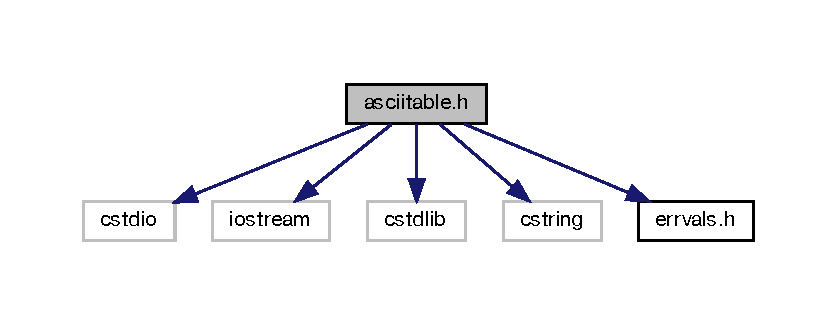
\includegraphics[width=350pt]{asciitable_8h__incl}
\end{center}
\end{figure}
\subsection*{Data Structures}
\begin{DoxyCompactItemize}
\item 
class \hyperlink{classASCIITable}{A\+S\+C\+I\+I\+Table}
\begin{DoxyCompactList}\small\item\em implements basic input/output operations on ascii table dataset \end{DoxyCompactList}\end{DoxyCompactItemize}
\subsection*{Macros}
\begin{DoxyCompactItemize}
\item 
\#define \hyperlink{asciitable_8h_ad3273464643b12407cb405d8c298f943}{L\+M\+A\+X\+S\+I\+ZE}~64 /$\ast$ max allowed line length $\ast$/
\item 
\#define \hyperlink{asciitable_8h_a7de6f71b3f223ff342d8517e2706252d}{F\+S\+I\+ZE}~16     /$\ast$ max allowed number of characters in a field (cell) include \textquotesingle{}\textbackslash{}0\textquotesingle{} $\ast$/
\item 
\#define \hyperlink{asciitable_8h_af9520fdf42fc2eb129de2c594eb10505}{F\+M\+AX}~16      /$\ast$ max allowed number of fields (columns) in a row $\ast$/
\item 
\#define \hyperlink{asciitable_8h_a66d21d4cc0d35bfe93b68f7a5089eb8b}{R\+M\+AX}~16      /$\ast$ max allowed number of records (rows) in a file $\ast$/
\item 
\#define \hyperlink{asciitable_8h_af8903d8eea3868940c60af887473b152}{RS}~\textquotesingle{}\textbackslash{}n\textquotesingle{}     /$\ast$ (input) record (row) separator $\ast$/
\item 
\#define \hyperlink{asciitable_8h_a30588c5eca7c9cb6ebba02a0236f0119}{FS}~\textquotesingle{} \textquotesingle{}     /$\ast$ (input) field (column) separator $\ast$/
\item 
\#define \hyperlink{asciitable_8h_aba177a1850218eefd2e7dcd37982926e}{O\+RS}~\textquotesingle{}\textbackslash{}n\textquotesingle{}     /$\ast$ output record (row) separator $\ast$/
\item 
\#define \hyperlink{asciitable_8h_a6a9fc425927b28770e853b880dd11c5b}{O\+FS}~\textquotesingle{},\textquotesingle{}     /$\ast$ output field (column) separator $\ast$/
\end{DoxyCompactItemize}


\subsection{Detailed Description}
(C) 2021 Francesco Lazzarotto  \href{mailto:francesco.lazzarotto@iaps.inaf.it}{\tt francesco.\+lazzarotto@iaps.\+inaf.\+it} \hyperlink{}{This program is free software\+: you can redistribute it and/or modify it under the terms of the G\+NU General Public License as published by the Free Software Foundation, either version 3 of the License, or (at your option) any later version. This program is distributed in the hope that it will be useful, but W\+I\+T\+H\+O\+UT A\+NY W\+A\+R\+R\+A\+N\+TY; without even the implied warranty of M\+E\+R\+C\+H\+A\+N\+T\+A\+B\+I\+L\+I\+TY or F\+I\+T\+N\+E\+SS F\+OR A P\+A\+R\+T\+I\+C\+U\+L\+AR P\+U\+R\+P\+O\+SE. See the G\+NU General Public License for more details. You should have received a copy of the G\+NU General Public License along with this program. If not, see  \href{http://www.gnu.org/licenses/}{\tt http\+://www.\+gnu.\+org/licenses/}. }

\subsection{Macro Definition Documentation}
\mbox{\Hypertarget{asciitable_8h_af9520fdf42fc2eb129de2c594eb10505}\label{asciitable_8h_af9520fdf42fc2eb129de2c594eb10505}} 
\index{asciitable.\+h@{asciitable.\+h}!F\+M\+AX@{F\+M\+AX}}
\index{F\+M\+AX@{F\+M\+AX}!asciitable.\+h@{asciitable.\+h}}
\subsubsection{\texorpdfstring{F\+M\+AX}{FMAX}}
{\footnotesize\ttfamily \#define F\+M\+AX~16      /$\ast$ max allowed number of fields (columns) in a row $\ast$/}

\mbox{\Hypertarget{asciitable_8h_a30588c5eca7c9cb6ebba02a0236f0119}\label{asciitable_8h_a30588c5eca7c9cb6ebba02a0236f0119}} 
\index{asciitable.\+h@{asciitable.\+h}!FS@{FS}}
\index{FS@{FS}!asciitable.\+h@{asciitable.\+h}}
\subsubsection{\texorpdfstring{FS}{FS}}
{\footnotesize\ttfamily \#define FS~\textquotesingle{} \textquotesingle{}     /$\ast$ (input) field (column) separator $\ast$/}

\mbox{\Hypertarget{asciitable_8h_a7de6f71b3f223ff342d8517e2706252d}\label{asciitable_8h_a7de6f71b3f223ff342d8517e2706252d}} 
\index{asciitable.\+h@{asciitable.\+h}!F\+S\+I\+ZE@{F\+S\+I\+ZE}}
\index{F\+S\+I\+ZE@{F\+S\+I\+ZE}!asciitable.\+h@{asciitable.\+h}}
\subsubsection{\texorpdfstring{F\+S\+I\+ZE}{FSIZE}}
{\footnotesize\ttfamily \#define F\+S\+I\+ZE~16     /$\ast$ max allowed number of characters in a field (cell) include \textquotesingle{}\textbackslash{}0\textquotesingle{} $\ast$/}

\mbox{\Hypertarget{asciitable_8h_ad3273464643b12407cb405d8c298f943}\label{asciitable_8h_ad3273464643b12407cb405d8c298f943}} 
\index{asciitable.\+h@{asciitable.\+h}!L\+M\+A\+X\+S\+I\+ZE@{L\+M\+A\+X\+S\+I\+ZE}}
\index{L\+M\+A\+X\+S\+I\+ZE@{L\+M\+A\+X\+S\+I\+ZE}!asciitable.\+h@{asciitable.\+h}}
\subsubsection{\texorpdfstring{L\+M\+A\+X\+S\+I\+ZE}{LMAXSIZE}}
{\footnotesize\ttfamily \#define L\+M\+A\+X\+S\+I\+ZE~64 /$\ast$ max allowed line length $\ast$/}

\mbox{\Hypertarget{asciitable_8h_a6a9fc425927b28770e853b880dd11c5b}\label{asciitable_8h_a6a9fc425927b28770e853b880dd11c5b}} 
\index{asciitable.\+h@{asciitable.\+h}!O\+FS@{O\+FS}}
\index{O\+FS@{O\+FS}!asciitable.\+h@{asciitable.\+h}}
\subsubsection{\texorpdfstring{O\+FS}{OFS}}
{\footnotesize\ttfamily \#define O\+FS~\textquotesingle{},\textquotesingle{}     /$\ast$ output field (column) separator $\ast$/}

\mbox{\Hypertarget{asciitable_8h_aba177a1850218eefd2e7dcd37982926e}\label{asciitable_8h_aba177a1850218eefd2e7dcd37982926e}} 
\index{asciitable.\+h@{asciitable.\+h}!O\+RS@{O\+RS}}
\index{O\+RS@{O\+RS}!asciitable.\+h@{asciitable.\+h}}
\subsubsection{\texorpdfstring{O\+RS}{ORS}}
{\footnotesize\ttfamily \#define O\+RS~\textquotesingle{}\textbackslash{}n\textquotesingle{}     /$\ast$ output record (row) separator $\ast$/}

\mbox{\Hypertarget{asciitable_8h_a66d21d4cc0d35bfe93b68f7a5089eb8b}\label{asciitable_8h_a66d21d4cc0d35bfe93b68f7a5089eb8b}} 
\index{asciitable.\+h@{asciitable.\+h}!R\+M\+AX@{R\+M\+AX}}
\index{R\+M\+AX@{R\+M\+AX}!asciitable.\+h@{asciitable.\+h}}
\subsubsection{\texorpdfstring{R\+M\+AX}{RMAX}}
{\footnotesize\ttfamily \#define R\+M\+AX~16      /$\ast$ max allowed number of records (rows) in a file $\ast$/}

\mbox{\Hypertarget{asciitable_8h_af8903d8eea3868940c60af887473b152}\label{asciitable_8h_af8903d8eea3868940c60af887473b152}} 
\index{asciitable.\+h@{asciitable.\+h}!RS@{RS}}
\index{RS@{RS}!asciitable.\+h@{asciitable.\+h}}
\subsubsection{\texorpdfstring{RS}{RS}}
{\footnotesize\ttfamily \#define RS~\textquotesingle{}\textbackslash{}n\textquotesingle{}     /$\ast$ (input) record (row) separator $\ast$/}


\hypertarget{defines_8h}{}\section{defines.\+h File Reference}
\label{defines_8h}\index{defines.\+h@{defines.\+h}}
{\ttfamily \#include $<$cstdio$>$}\newline
{\ttfamily \#include $<$cstdlib$>$}\newline
{\ttfamily \#include $<$cstring$>$}\newline
{\ttfamily \#include \char`\"{}errvals.\+h\char`\"{}}\newline
Include dependency graph for defines.\+h\+:\nopagebreak
\begin{figure}[H]
\begin{center}
\leavevmode
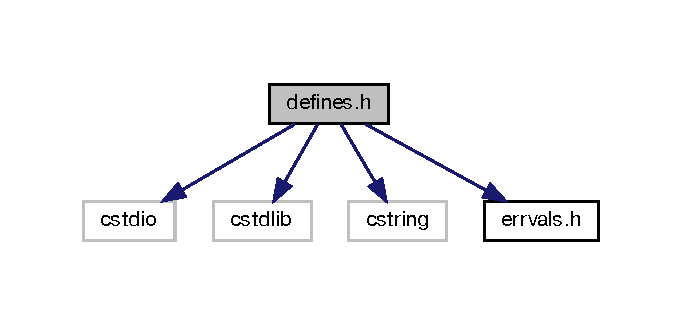
\includegraphics[width=328pt]{defines_8h__incl}
\end{center}
\end{figure}

\hypertarget{errvals_8h}{}\section{errvals.\+h File Reference}
\label{errvals_8h}\index{errvals.\+h@{errvals.\+h}}
This graph shows which files directly or indirectly include this file\+:\nopagebreak
\begin{figure}[H]
\begin{center}
\leavevmode
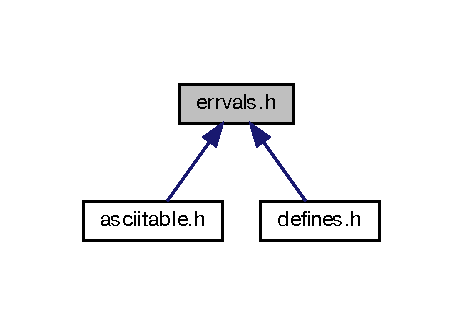
\includegraphics[width=222pt]{errvals_8h__dep__incl}
\end{center}
\end{figure}
\subsection*{Macros}
\begin{DoxyCompactItemize}
\item 
\#define \hyperlink{errvals_8h_aed4bd849f99a5328fe36d1963de00591}{E\+X\+\_\+\+OK}~0	/$\ast$$\ast$ successful termination $\ast$/
\item 
\#define \hyperlink{errvals_8h_a5801735e57b4c6554d4124742da8e8df}{E\+X\+\_\+\+S\+Y\+N\+E\+RR}~2	/$\ast$$\ast$ syntax error $\ast$/
\item 
\#define \hyperlink{errvals_8h_aaed0821130d25b0086d3b0c0ca150278}{E\+X\+\_\+\+\_\+\+B\+A\+SE}~64	/$\ast$$\ast$ base value for error messages $\ast$/
\item 
\#define \hyperlink{errvals_8h_abbdf9290893d2876419c13b7b28f5d4e}{E\+X\+\_\+\+U\+S\+A\+GE}~64	/$\ast$$\ast$ command line usage error $\ast$/
\item 
\#define \hyperlink{errvals_8h_a483a5c14de098f6fc02950fbeb3cab5e}{E\+X\+\_\+\+D\+A\+T\+A\+E\+RR}~65	/$\ast$$\ast$ data format error $\ast$/
\item 
\#define \hyperlink{errvals_8h_aee8a9f0cf8b09e7734b9c5c4f75218cf}{E\+X\+\_\+\+N\+O\+I\+N\+P\+UT}~66	/$\ast$$\ast$ cannot open input $\ast$/
\item 
\#define \hyperlink{errvals_8h_a9b187a247bf7757c06cd1c629bfe0a8a}{E\+X\+\_\+\+N\+O\+U\+S\+ER}~67	/$\ast$$\ast$ addressee unknown $\ast$/
\item 
\#define \hyperlink{errvals_8h_a8e7a847198a05d6192733d2636b07005}{E\+X\+\_\+\+N\+O\+H\+O\+ST}~68	/$\ast$$\ast$ host name unknown $\ast$/
\item 
\#define \hyperlink{errvals_8h_a64700ca081061c72709f72adb438be49}{E\+X\+\_\+\+U\+N\+A\+V\+A\+I\+L\+A\+B\+LE}~69	/$\ast$$\ast$ service unavailable $\ast$/
\item 
\#define \hyperlink{errvals_8h_a587ae77ee5b3c931c10cb51c19053f11}{E\+X\+\_\+\+S\+O\+F\+T\+W\+A\+RE}~70	/$\ast$$\ast$ internal software error $\ast$/
\item 
\#define \hyperlink{errvals_8h_aa88a6d093c89b8d7e868fc6baa0a214a}{E\+X\+\_\+\+O\+S\+E\+RR}~71	/$\ast$$\ast$ system error (e.\+g., can\textquotesingle{}t fork) $\ast$/
\item 
\#define \hyperlink{errvals_8h_a8420ff74ab88b08df924ccab61ec2e6e}{E\+X\+\_\+\+O\+S\+F\+I\+LE}~72	/$\ast$$\ast$ critical OS file missing $\ast$/
\item 
\#define \hyperlink{errvals_8h_ac030cfddafe98bacd8db830a75f81f03}{E\+X\+\_\+\+C\+A\+N\+T\+C\+R\+E\+AT}~73	/$\ast$$\ast$ can\textquotesingle{}t create (user) output file $\ast$/
\item 
\#define \hyperlink{errvals_8h_a51dc7f5948835cdf92471f9478fab3ff}{E\+X\+\_\+\+I\+O\+E\+RR}~74	/$\ast$$\ast$ input/output error $\ast$/
\item 
\#define \hyperlink{errvals_8h_a0143ccd308d239d00953b99b265e8deb}{E\+X\+\_\+\+T\+E\+M\+P\+F\+A\+IL}~75	/$\ast$$\ast$ temp failure; user is invited to retry $\ast$/
\item 
\#define \hyperlink{errvals_8h_ab781475747a100ce2cbaaa57c9c45fe9}{E\+X\+\_\+\+P\+R\+O\+T\+O\+C\+OL}~76	/$\ast$$\ast$ remote error in protocol $\ast$/
\item 
\#define \hyperlink{errvals_8h_af091b7431988e6ca8e3a2949ec82f7b0}{E\+X\+\_\+\+N\+O\+P\+E\+RM}~77	/$\ast$$\ast$ permission denied $\ast$/
\item 
\#define \hyperlink{errvals_8h_a060f7b1fcb099e3bbebf729050ba9414}{E\+X\+\_\+\+C\+O\+N\+F\+IG}~78	/$\ast$$\ast$ configuration error $\ast$/
\item 
\#define \hyperlink{errvals_8h_a7628ad7a1ca09fe4137a2f8ebff01558}{E\+X\+\_\+\+\_\+\+M\+AX}~79	/$\ast$$\ast$ maximum listed value $\ast$/
\item 
\#define \hyperlink{errvals_8h_af46e83836e145e4123b00697b9828e02}{E\+X\+\_\+\+B\+A\+D\+A\+R\+GS}~85         /$\ast$$\ast$ Wrong number of arguments $\ast$/
\item 
\#define \hyperlink{errvals_8h_a90d8ad14c2192d5d6af88ba2830187be}{E\+X\+\_\+\+A\+R\+G\+S\+L\+I\+M\+I\+TS}~86      /$\ast$$\ast$ an argument is out of allowed limits $\ast$/
\item 
\#define \hyperlink{errvals_8h_aa7a7fea7c9887f575533977feccd94c6}{E\+X\+\_\+\+U\+N\+S\+U\+P\+P\+O\+R\+T\+ED}~87     /$\ast$$\ast$ unsupported system $\ast$/
\item 
\#define \hyperlink{errvals_8h_a650d1e9c575b5f3b210ce4b3abe4e54a}{E\+X\+\_\+\+D\+E\+N\+I\+ED}~126      /$\ast$$\ast$ permission denied $\ast$/
\item 
\#define \hyperlink{errvals_8h_a8918dc5d9bb418fe96c77851b86887d1}{E\+X\+\_\+\+N\+O\+F\+I\+LE}~127     /$\ast$$\ast$ file not present $\ast$/
\item 
\#define \hyperlink{errvals_8h_accb9d6ca49394b476a27d17451c78b62}{E\+X\+\_\+\+S\+E\+G\+F\+A\+U\+LT}~139     /$\ast$$\ast$ access to not allowed memory $\ast$/
\end{DoxyCompactItemize}
\subsection*{Functions}
\begin{DoxyCompactItemize}
\item 
void \hyperlink{errvals_8h_a0723fcf97b6950d25e2c653313093442}{error\+\_\+what} (int eid)
\begin{DoxyCompactList}\small\item\em gives the error message in function of the error code \end{DoxyCompactList}\end{DoxyCompactItemize}


\subsection{Macro Definition Documentation}
\mbox{\Hypertarget{errvals_8h_aaed0821130d25b0086d3b0c0ca150278}\label{errvals_8h_aaed0821130d25b0086d3b0c0ca150278}} 
\index{errvals.\+h@{errvals.\+h}!E\+X\+\_\+\+\_\+\+B\+A\+SE@{E\+X\+\_\+\+\_\+\+B\+A\+SE}}
\index{E\+X\+\_\+\+\_\+\+B\+A\+SE@{E\+X\+\_\+\+\_\+\+B\+A\+SE}!errvals.\+h@{errvals.\+h}}
\subsubsection{\texorpdfstring{E\+X\+\_\+\+\_\+\+B\+A\+SE}{EX\_\_BASE}}
{\footnotesize\ttfamily \#define E\+X\+\_\+\+\_\+\+B\+A\+SE~64	/$\ast$$\ast$ base value for error messages $\ast$/}

\mbox{\Hypertarget{errvals_8h_a7628ad7a1ca09fe4137a2f8ebff01558}\label{errvals_8h_a7628ad7a1ca09fe4137a2f8ebff01558}} 
\index{errvals.\+h@{errvals.\+h}!E\+X\+\_\+\+\_\+\+M\+AX@{E\+X\+\_\+\+\_\+\+M\+AX}}
\index{E\+X\+\_\+\+\_\+\+M\+AX@{E\+X\+\_\+\+\_\+\+M\+AX}!errvals.\+h@{errvals.\+h}}
\subsubsection{\texorpdfstring{E\+X\+\_\+\+\_\+\+M\+AX}{EX\_\_MAX}}
{\footnotesize\ttfamily \#define E\+X\+\_\+\+\_\+\+M\+AX~79	/$\ast$$\ast$ maximum listed value $\ast$/}

\mbox{\Hypertarget{errvals_8h_a90d8ad14c2192d5d6af88ba2830187be}\label{errvals_8h_a90d8ad14c2192d5d6af88ba2830187be}} 
\index{errvals.\+h@{errvals.\+h}!E\+X\+\_\+\+A\+R\+G\+S\+L\+I\+M\+I\+TS@{E\+X\+\_\+\+A\+R\+G\+S\+L\+I\+M\+I\+TS}}
\index{E\+X\+\_\+\+A\+R\+G\+S\+L\+I\+M\+I\+TS@{E\+X\+\_\+\+A\+R\+G\+S\+L\+I\+M\+I\+TS}!errvals.\+h@{errvals.\+h}}
\subsubsection{\texorpdfstring{E\+X\+\_\+\+A\+R\+G\+S\+L\+I\+M\+I\+TS}{EX\_ARGSLIMITS}}
{\footnotesize\ttfamily \#define E\+X\+\_\+\+A\+R\+G\+S\+L\+I\+M\+I\+TS~86      /$\ast$$\ast$ an argument is out of allowed limits $\ast$/}

\mbox{\Hypertarget{errvals_8h_af46e83836e145e4123b00697b9828e02}\label{errvals_8h_af46e83836e145e4123b00697b9828e02}} 
\index{errvals.\+h@{errvals.\+h}!E\+X\+\_\+\+B\+A\+D\+A\+R\+GS@{E\+X\+\_\+\+B\+A\+D\+A\+R\+GS}}
\index{E\+X\+\_\+\+B\+A\+D\+A\+R\+GS@{E\+X\+\_\+\+B\+A\+D\+A\+R\+GS}!errvals.\+h@{errvals.\+h}}
\subsubsection{\texorpdfstring{E\+X\+\_\+\+B\+A\+D\+A\+R\+GS}{EX\_BADARGS}}
{\footnotesize\ttfamily \#define E\+X\+\_\+\+B\+A\+D\+A\+R\+GS~85         /$\ast$$\ast$ Wrong number of arguments $\ast$/}

mendel cooper abs guide example exit codes \mbox{\Hypertarget{errvals_8h_ac030cfddafe98bacd8db830a75f81f03}\label{errvals_8h_ac030cfddafe98bacd8db830a75f81f03}} 
\index{errvals.\+h@{errvals.\+h}!E\+X\+\_\+\+C\+A\+N\+T\+C\+R\+E\+AT@{E\+X\+\_\+\+C\+A\+N\+T\+C\+R\+E\+AT}}
\index{E\+X\+\_\+\+C\+A\+N\+T\+C\+R\+E\+AT@{E\+X\+\_\+\+C\+A\+N\+T\+C\+R\+E\+AT}!errvals.\+h@{errvals.\+h}}
\subsubsection{\texorpdfstring{E\+X\+\_\+\+C\+A\+N\+T\+C\+R\+E\+AT}{EX\_CANTCREAT}}
{\footnotesize\ttfamily \#define E\+X\+\_\+\+C\+A\+N\+T\+C\+R\+E\+AT~73	/$\ast$$\ast$ can\textquotesingle{}t create (user) output file $\ast$/}

\mbox{\Hypertarget{errvals_8h_a060f7b1fcb099e3bbebf729050ba9414}\label{errvals_8h_a060f7b1fcb099e3bbebf729050ba9414}} 
\index{errvals.\+h@{errvals.\+h}!E\+X\+\_\+\+C\+O\+N\+F\+IG@{E\+X\+\_\+\+C\+O\+N\+F\+IG}}
\index{E\+X\+\_\+\+C\+O\+N\+F\+IG@{E\+X\+\_\+\+C\+O\+N\+F\+IG}!errvals.\+h@{errvals.\+h}}
\subsubsection{\texorpdfstring{E\+X\+\_\+\+C\+O\+N\+F\+IG}{EX\_CONFIG}}
{\footnotesize\ttfamily \#define E\+X\+\_\+\+C\+O\+N\+F\+IG~78	/$\ast$$\ast$ configuration error $\ast$/}

\mbox{\Hypertarget{errvals_8h_a483a5c14de098f6fc02950fbeb3cab5e}\label{errvals_8h_a483a5c14de098f6fc02950fbeb3cab5e}} 
\index{errvals.\+h@{errvals.\+h}!E\+X\+\_\+\+D\+A\+T\+A\+E\+RR@{E\+X\+\_\+\+D\+A\+T\+A\+E\+RR}}
\index{E\+X\+\_\+\+D\+A\+T\+A\+E\+RR@{E\+X\+\_\+\+D\+A\+T\+A\+E\+RR}!errvals.\+h@{errvals.\+h}}
\subsubsection{\texorpdfstring{E\+X\+\_\+\+D\+A\+T\+A\+E\+RR}{EX\_DATAERR}}
{\footnotesize\ttfamily \#define E\+X\+\_\+\+D\+A\+T\+A\+E\+RR~65	/$\ast$$\ast$ data format error $\ast$/}

\mbox{\Hypertarget{errvals_8h_a650d1e9c575b5f3b210ce4b3abe4e54a}\label{errvals_8h_a650d1e9c575b5f3b210ce4b3abe4e54a}} 
\index{errvals.\+h@{errvals.\+h}!E\+X\+\_\+\+D\+E\+N\+I\+ED@{E\+X\+\_\+\+D\+E\+N\+I\+ED}}
\index{E\+X\+\_\+\+D\+E\+N\+I\+ED@{E\+X\+\_\+\+D\+E\+N\+I\+ED}!errvals.\+h@{errvals.\+h}}
\subsubsection{\texorpdfstring{E\+X\+\_\+\+D\+E\+N\+I\+ED}{EX\_DENIED}}
{\footnotesize\ttfamily \#define E\+X\+\_\+\+D\+E\+N\+I\+ED~126      /$\ast$$\ast$ permission denied $\ast$/}

system exit values \mbox{\Hypertarget{errvals_8h_a51dc7f5948835cdf92471f9478fab3ff}\label{errvals_8h_a51dc7f5948835cdf92471f9478fab3ff}} 
\index{errvals.\+h@{errvals.\+h}!E\+X\+\_\+\+I\+O\+E\+RR@{E\+X\+\_\+\+I\+O\+E\+RR}}
\index{E\+X\+\_\+\+I\+O\+E\+RR@{E\+X\+\_\+\+I\+O\+E\+RR}!errvals.\+h@{errvals.\+h}}
\subsubsection{\texorpdfstring{E\+X\+\_\+\+I\+O\+E\+RR}{EX\_IOERR}}
{\footnotesize\ttfamily \#define E\+X\+\_\+\+I\+O\+E\+RR~74	/$\ast$$\ast$ input/output error $\ast$/}

\mbox{\Hypertarget{errvals_8h_a8918dc5d9bb418fe96c77851b86887d1}\label{errvals_8h_a8918dc5d9bb418fe96c77851b86887d1}} 
\index{errvals.\+h@{errvals.\+h}!E\+X\+\_\+\+N\+O\+F\+I\+LE@{E\+X\+\_\+\+N\+O\+F\+I\+LE}}
\index{E\+X\+\_\+\+N\+O\+F\+I\+LE@{E\+X\+\_\+\+N\+O\+F\+I\+LE}!errvals.\+h@{errvals.\+h}}
\subsubsection{\texorpdfstring{E\+X\+\_\+\+N\+O\+F\+I\+LE}{EX\_NOFILE}}
{\footnotesize\ttfamily \#define E\+X\+\_\+\+N\+O\+F\+I\+LE~127     /$\ast$$\ast$ file not present $\ast$/}

\mbox{\Hypertarget{errvals_8h_a8e7a847198a05d6192733d2636b07005}\label{errvals_8h_a8e7a847198a05d6192733d2636b07005}} 
\index{errvals.\+h@{errvals.\+h}!E\+X\+\_\+\+N\+O\+H\+O\+ST@{E\+X\+\_\+\+N\+O\+H\+O\+ST}}
\index{E\+X\+\_\+\+N\+O\+H\+O\+ST@{E\+X\+\_\+\+N\+O\+H\+O\+ST}!errvals.\+h@{errvals.\+h}}
\subsubsection{\texorpdfstring{E\+X\+\_\+\+N\+O\+H\+O\+ST}{EX\_NOHOST}}
{\footnotesize\ttfamily \#define E\+X\+\_\+\+N\+O\+H\+O\+ST~68	/$\ast$$\ast$ host name unknown $\ast$/}

\mbox{\Hypertarget{errvals_8h_aee8a9f0cf8b09e7734b9c5c4f75218cf}\label{errvals_8h_aee8a9f0cf8b09e7734b9c5c4f75218cf}} 
\index{errvals.\+h@{errvals.\+h}!E\+X\+\_\+\+N\+O\+I\+N\+P\+UT@{E\+X\+\_\+\+N\+O\+I\+N\+P\+UT}}
\index{E\+X\+\_\+\+N\+O\+I\+N\+P\+UT@{E\+X\+\_\+\+N\+O\+I\+N\+P\+UT}!errvals.\+h@{errvals.\+h}}
\subsubsection{\texorpdfstring{E\+X\+\_\+\+N\+O\+I\+N\+P\+UT}{EX\_NOINPUT}}
{\footnotesize\ttfamily \#define E\+X\+\_\+\+N\+O\+I\+N\+P\+UT~66	/$\ast$$\ast$ cannot open input $\ast$/}

\mbox{\Hypertarget{errvals_8h_af091b7431988e6ca8e3a2949ec82f7b0}\label{errvals_8h_af091b7431988e6ca8e3a2949ec82f7b0}} 
\index{errvals.\+h@{errvals.\+h}!E\+X\+\_\+\+N\+O\+P\+E\+RM@{E\+X\+\_\+\+N\+O\+P\+E\+RM}}
\index{E\+X\+\_\+\+N\+O\+P\+E\+RM@{E\+X\+\_\+\+N\+O\+P\+E\+RM}!errvals.\+h@{errvals.\+h}}
\subsubsection{\texorpdfstring{E\+X\+\_\+\+N\+O\+P\+E\+RM}{EX\_NOPERM}}
{\footnotesize\ttfamily \#define E\+X\+\_\+\+N\+O\+P\+E\+RM~77	/$\ast$$\ast$ permission denied $\ast$/}

\mbox{\Hypertarget{errvals_8h_a9b187a247bf7757c06cd1c629bfe0a8a}\label{errvals_8h_a9b187a247bf7757c06cd1c629bfe0a8a}} 
\index{errvals.\+h@{errvals.\+h}!E\+X\+\_\+\+N\+O\+U\+S\+ER@{E\+X\+\_\+\+N\+O\+U\+S\+ER}}
\index{E\+X\+\_\+\+N\+O\+U\+S\+ER@{E\+X\+\_\+\+N\+O\+U\+S\+ER}!errvals.\+h@{errvals.\+h}}
\subsubsection{\texorpdfstring{E\+X\+\_\+\+N\+O\+U\+S\+ER}{EX\_NOUSER}}
{\footnotesize\ttfamily \#define E\+X\+\_\+\+N\+O\+U\+S\+ER~67	/$\ast$$\ast$ addressee unknown $\ast$/}

\mbox{\Hypertarget{errvals_8h_aed4bd849f99a5328fe36d1963de00591}\label{errvals_8h_aed4bd849f99a5328fe36d1963de00591}} 
\index{errvals.\+h@{errvals.\+h}!E\+X\+\_\+\+OK@{E\+X\+\_\+\+OK}}
\index{E\+X\+\_\+\+OK@{E\+X\+\_\+\+OK}!errvals.\+h@{errvals.\+h}}
\subsubsection{\texorpdfstring{E\+X\+\_\+\+OK}{EX\_OK}}
{\footnotesize\ttfamily \#define E\+X\+\_\+\+OK~0	/$\ast$$\ast$ successful termination $\ast$/}

\mbox{\Hypertarget{errvals_8h_aa88a6d093c89b8d7e868fc6baa0a214a}\label{errvals_8h_aa88a6d093c89b8d7e868fc6baa0a214a}} 
\index{errvals.\+h@{errvals.\+h}!E\+X\+\_\+\+O\+S\+E\+RR@{E\+X\+\_\+\+O\+S\+E\+RR}}
\index{E\+X\+\_\+\+O\+S\+E\+RR@{E\+X\+\_\+\+O\+S\+E\+RR}!errvals.\+h@{errvals.\+h}}
\subsubsection{\texorpdfstring{E\+X\+\_\+\+O\+S\+E\+RR}{EX\_OSERR}}
{\footnotesize\ttfamily \#define E\+X\+\_\+\+O\+S\+E\+RR~71	/$\ast$$\ast$ system error (e.\+g., can\textquotesingle{}t fork) $\ast$/}

\mbox{\Hypertarget{errvals_8h_a8420ff74ab88b08df924ccab61ec2e6e}\label{errvals_8h_a8420ff74ab88b08df924ccab61ec2e6e}} 
\index{errvals.\+h@{errvals.\+h}!E\+X\+\_\+\+O\+S\+F\+I\+LE@{E\+X\+\_\+\+O\+S\+F\+I\+LE}}
\index{E\+X\+\_\+\+O\+S\+F\+I\+LE@{E\+X\+\_\+\+O\+S\+F\+I\+LE}!errvals.\+h@{errvals.\+h}}
\subsubsection{\texorpdfstring{E\+X\+\_\+\+O\+S\+F\+I\+LE}{EX\_OSFILE}}
{\footnotesize\ttfamily \#define E\+X\+\_\+\+O\+S\+F\+I\+LE~72	/$\ast$$\ast$ critical OS file missing $\ast$/}

\mbox{\Hypertarget{errvals_8h_ab781475747a100ce2cbaaa57c9c45fe9}\label{errvals_8h_ab781475747a100ce2cbaaa57c9c45fe9}} 
\index{errvals.\+h@{errvals.\+h}!E\+X\+\_\+\+P\+R\+O\+T\+O\+C\+OL@{E\+X\+\_\+\+P\+R\+O\+T\+O\+C\+OL}}
\index{E\+X\+\_\+\+P\+R\+O\+T\+O\+C\+OL@{E\+X\+\_\+\+P\+R\+O\+T\+O\+C\+OL}!errvals.\+h@{errvals.\+h}}
\subsubsection{\texorpdfstring{E\+X\+\_\+\+P\+R\+O\+T\+O\+C\+OL}{EX\_PROTOCOL}}
{\footnotesize\ttfamily \#define E\+X\+\_\+\+P\+R\+O\+T\+O\+C\+OL~76	/$\ast$$\ast$ remote error in protocol $\ast$/}

\mbox{\Hypertarget{errvals_8h_accb9d6ca49394b476a27d17451c78b62}\label{errvals_8h_accb9d6ca49394b476a27d17451c78b62}} 
\index{errvals.\+h@{errvals.\+h}!E\+X\+\_\+\+S\+E\+G\+F\+A\+U\+LT@{E\+X\+\_\+\+S\+E\+G\+F\+A\+U\+LT}}
\index{E\+X\+\_\+\+S\+E\+G\+F\+A\+U\+LT@{E\+X\+\_\+\+S\+E\+G\+F\+A\+U\+LT}!errvals.\+h@{errvals.\+h}}
\subsubsection{\texorpdfstring{E\+X\+\_\+\+S\+E\+G\+F\+A\+U\+LT}{EX\_SEGFAULT}}
{\footnotesize\ttfamily \#define E\+X\+\_\+\+S\+E\+G\+F\+A\+U\+LT~139     /$\ast$$\ast$ access to not allowed memory $\ast$/}

\mbox{\Hypertarget{errvals_8h_a587ae77ee5b3c931c10cb51c19053f11}\label{errvals_8h_a587ae77ee5b3c931c10cb51c19053f11}} 
\index{errvals.\+h@{errvals.\+h}!E\+X\+\_\+\+S\+O\+F\+T\+W\+A\+RE@{E\+X\+\_\+\+S\+O\+F\+T\+W\+A\+RE}}
\index{E\+X\+\_\+\+S\+O\+F\+T\+W\+A\+RE@{E\+X\+\_\+\+S\+O\+F\+T\+W\+A\+RE}!errvals.\+h@{errvals.\+h}}
\subsubsection{\texorpdfstring{E\+X\+\_\+\+S\+O\+F\+T\+W\+A\+RE}{EX\_SOFTWARE}}
{\footnotesize\ttfamily \#define E\+X\+\_\+\+S\+O\+F\+T\+W\+A\+RE~70	/$\ast$$\ast$ internal software error $\ast$/}

\mbox{\Hypertarget{errvals_8h_a5801735e57b4c6554d4124742da8e8df}\label{errvals_8h_a5801735e57b4c6554d4124742da8e8df}} 
\index{errvals.\+h@{errvals.\+h}!E\+X\+\_\+\+S\+Y\+N\+E\+RR@{E\+X\+\_\+\+S\+Y\+N\+E\+RR}}
\index{E\+X\+\_\+\+S\+Y\+N\+E\+RR@{E\+X\+\_\+\+S\+Y\+N\+E\+RR}!errvals.\+h@{errvals.\+h}}
\subsubsection{\texorpdfstring{E\+X\+\_\+\+S\+Y\+N\+E\+RR}{EX\_SYNERR}}
{\footnotesize\ttfamily \#define E\+X\+\_\+\+S\+Y\+N\+E\+RR~2	/$\ast$$\ast$ syntax error $\ast$/}

\mbox{\Hypertarget{errvals_8h_a0143ccd308d239d00953b99b265e8deb}\label{errvals_8h_a0143ccd308d239d00953b99b265e8deb}} 
\index{errvals.\+h@{errvals.\+h}!E\+X\+\_\+\+T\+E\+M\+P\+F\+A\+IL@{E\+X\+\_\+\+T\+E\+M\+P\+F\+A\+IL}}
\index{E\+X\+\_\+\+T\+E\+M\+P\+F\+A\+IL@{E\+X\+\_\+\+T\+E\+M\+P\+F\+A\+IL}!errvals.\+h@{errvals.\+h}}
\subsubsection{\texorpdfstring{E\+X\+\_\+\+T\+E\+M\+P\+F\+A\+IL}{EX\_TEMPFAIL}}
{\footnotesize\ttfamily \#define E\+X\+\_\+\+T\+E\+M\+P\+F\+A\+IL~75	/$\ast$$\ast$ temp failure; user is invited to retry $\ast$/}

\mbox{\Hypertarget{errvals_8h_a64700ca081061c72709f72adb438be49}\label{errvals_8h_a64700ca081061c72709f72adb438be49}} 
\index{errvals.\+h@{errvals.\+h}!E\+X\+\_\+\+U\+N\+A\+V\+A\+I\+L\+A\+B\+LE@{E\+X\+\_\+\+U\+N\+A\+V\+A\+I\+L\+A\+B\+LE}}
\index{E\+X\+\_\+\+U\+N\+A\+V\+A\+I\+L\+A\+B\+LE@{E\+X\+\_\+\+U\+N\+A\+V\+A\+I\+L\+A\+B\+LE}!errvals.\+h@{errvals.\+h}}
\subsubsection{\texorpdfstring{E\+X\+\_\+\+U\+N\+A\+V\+A\+I\+L\+A\+B\+LE}{EX\_UNAVAILABLE}}
{\footnotesize\ttfamily \#define E\+X\+\_\+\+U\+N\+A\+V\+A\+I\+L\+A\+B\+LE~69	/$\ast$$\ast$ service unavailable $\ast$/}

\mbox{\Hypertarget{errvals_8h_aa7a7fea7c9887f575533977feccd94c6}\label{errvals_8h_aa7a7fea7c9887f575533977feccd94c6}} 
\index{errvals.\+h@{errvals.\+h}!E\+X\+\_\+\+U\+N\+S\+U\+P\+P\+O\+R\+T\+ED@{E\+X\+\_\+\+U\+N\+S\+U\+P\+P\+O\+R\+T\+ED}}
\index{E\+X\+\_\+\+U\+N\+S\+U\+P\+P\+O\+R\+T\+ED@{E\+X\+\_\+\+U\+N\+S\+U\+P\+P\+O\+R\+T\+ED}!errvals.\+h@{errvals.\+h}}
\subsubsection{\texorpdfstring{E\+X\+\_\+\+U\+N\+S\+U\+P\+P\+O\+R\+T\+ED}{EX\_UNSUPPORTED}}
{\footnotesize\ttfamily \#define E\+X\+\_\+\+U\+N\+S\+U\+P\+P\+O\+R\+T\+ED~87     /$\ast$$\ast$ unsupported system $\ast$/}

\mbox{\Hypertarget{errvals_8h_abbdf9290893d2876419c13b7b28f5d4e}\label{errvals_8h_abbdf9290893d2876419c13b7b28f5d4e}} 
\index{errvals.\+h@{errvals.\+h}!E\+X\+\_\+\+U\+S\+A\+GE@{E\+X\+\_\+\+U\+S\+A\+GE}}
\index{E\+X\+\_\+\+U\+S\+A\+GE@{E\+X\+\_\+\+U\+S\+A\+GE}!errvals.\+h@{errvals.\+h}}
\subsubsection{\texorpdfstring{E\+X\+\_\+\+U\+S\+A\+GE}{EX\_USAGE}}
{\footnotesize\ttfamily \#define E\+X\+\_\+\+U\+S\+A\+GE~64	/$\ast$$\ast$ command line usage error $\ast$/}



\subsection{Function Documentation}
\mbox{\Hypertarget{errvals_8h_a0723fcf97b6950d25e2c653313093442}\label{errvals_8h_a0723fcf97b6950d25e2c653313093442}} 
\index{errvals.\+h@{errvals.\+h}!error\+\_\+what@{error\+\_\+what}}
\index{error\+\_\+what@{error\+\_\+what}!errvals.\+h@{errvals.\+h}}
\subsubsection{\texorpdfstring{error\+\_\+what()}{error\_what()}}
{\footnotesize\ttfamily void error\+\_\+what (\begin{DoxyParamCaption}\item[{int}]{eid }\end{DoxyParamCaption})}



gives the error message in function of the error code 


%--- End generated contents ---

% Index
\backmatter
\newpage
\phantomsection
\clearemptydoublepage
\addcontentsline{toc}{chapter}{Index}
\printindex

\end{document}
